
\subsubsection{Diagrammi di sequenza}
Di seguito vengono riportati i diagrammi di sequenza.
\begin{figure}[H]
	\centering
	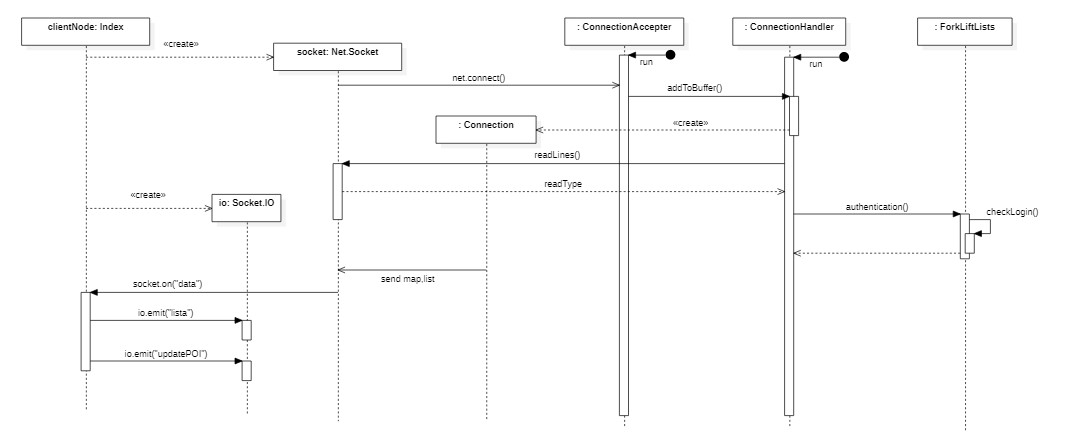
\includegraphics[scale=0.55]{res/diagrams/sequenza/connect unit.jpg}
	\caption{Visione complessiva della connessione server Java - unità muletto in NodeJS}
\end{figure}
Questo diagramma di sequenza rappresenta la prima connessione tra un'unità muletto in NodeJS e il server Java, attraverso il TCPsocket.
Nel diagramma viene raffigurato anche un socket.IO, che mette in comunicazione NodeJS con l'interfaccia grafica realizzata in Angular (non rappresentata nel diagramma).
\begin{figure}[H]
	\centering
	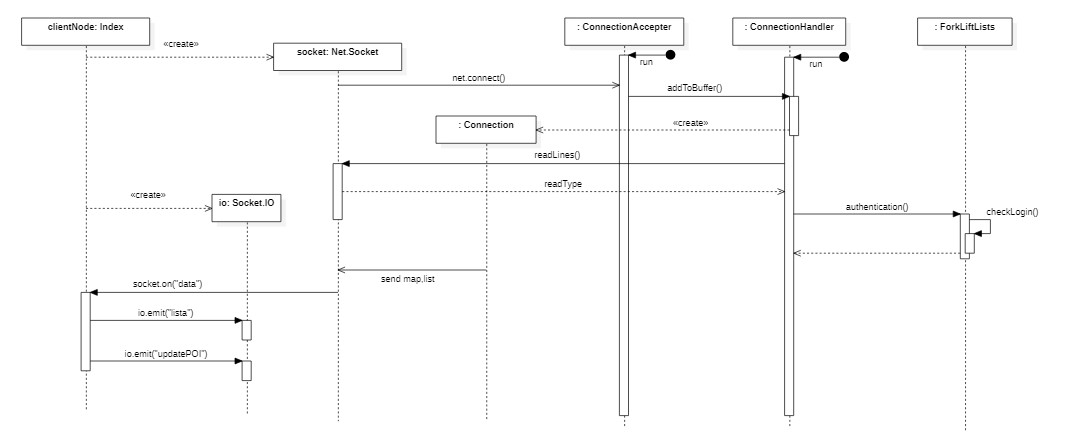
\includegraphics[scale=0.55]{res/diagrams/sequenza/connect unit.jpg}
	\caption{Esempio di comunicazione tra server e client, attraverso i socket TCP}
\end{figure}
Questo diagramma rappresenta un esempio di comunicazione tra server e client di tipo muletto. Il server legge i dati inviati dal muletto e invia una risposta, il muletto aggiorna l'interfaccia grafica in base alla risposta ricevuta dal server.